This section describes the two control-plane software systems, OESS and OSCARS. OESS is an OpenFlow controller
that accepts user advance-reservation requests for L2 paths
(in which start time, rate, duration, and endpoints are specified), performs intra-domain path computation, and configures rules in the switches along the path for VLAN based
packet forwarding using OpenFlow. OSCARS performs similar functions, and additionally supports inter-domain path
reservations and provisioning. Also, it can communicate
with a variety of switches/routers including some that do not
implement OpenFlow. Both OSCARS and OESS offer users
a Web Browser User Interface (UI) and a programmatic Web Service Interface for applications. In this section, we briefly
review the functionality offered by these controllers.
OESS supports integration with OSCARS, specifically to support inter-domain circuits.

\subsection{On-Demand Secure Circuits and Advance Reservation System (OSCARS)}
We review the overall OSCARS architecture, describe how trust/peering relationships are established between neighbouring OSCARS, and how topology is discovered before presenting how OSCARS reserves resources and provisions and releases paths (which is its main role). We end with a short review of path computation, which is executed during resource reservation \cite{OSCARS}.

\paragraph{Software architecture}
The OSCARS software consists of 11 modules that have distinct functions such as authentication, authorization, path finding, messaging, hardware mediation, and process coordination. Today, OSCARS supports inter-domain L2 paths using both the Inter-Domain Controller Protocol (IDCP) \cite{IDCP} and Network Service Interface Connection Services (NSI CS) version 2.0 \cite{NSI} protocols. The authorization (i.e., policy enforcement) of guaranteed bandwidth reservation requests are domain specific and can be enforced using the policy path computation modules within the OSCARS v0.6 Path Computation Engine (PCE) framework.

\paragraph{Trust/peering relationships}
The current trust model for
inter-domain dynamic paths is based on transitive peer-to-peer authentication and authorization. This work-flow mimics the telecommunication industry model; neither require downstream providers to know anything about the originating caller.

\paragraph{Topology discovery}
Each domain is responsible for discovering and pushing its topology to the perfSONAR Topology Service (pS-TS). The distributed pS-TS maintains
global topology information, and OSCARS servers can pull
the latest information from pS-TS as needed in real-time.
Topology information must be formatted in either the Open
Grid Forum Network Markup Language (NML) \cite{van2013network} or the NM-Control Plane \cite{IDCP} schemas to support the NSI CS v2.0
and the IDCP protocols, respectively.

\paragraph{Inter-domain L2 path reservation, provisioning, and
release}
When the OSCARS server in a domain receives an inter-domain VC reservation request, it reserves resources within its
own domain and sends a \texttt{createReservation} message
with endpoints, rate, start time (advance-reservation support)
and duration, to the OSCARS in the next domain, which is
selected based on the computed path. The procedure is executed in a daisy-chain fashion, as shown in Fig.~\ref{fig:daisychain},
until the OSCARS of the last domain on
the end-to-end path is reached. If successful, \texttt{Confirmation}
events are sent from one domain’s OSCARS server to the next
in the reverse direction. Provisioning of the VC occurs either
automatically or upon receiving a \texttt{createPath} message
from the user just before the reservation start-time. This procedure also uses a daisy-chain of signaling messages between
OSCARS servers. Each OSCARS server communicates with
the switches in its domain to provision the VC across the
domain. Finally, when the reservation end-time is reached a
\texttt{teardownPath} message is sent in daisy-chained mode to
release the VC.

The current trust model for inter-domain dynamic paths is based on transitive peer-to-peer authentication and authorization. This work-flow mimics the telecommunication industry model; neither require downstream providers to know anything about the originating caller.
\begin{figure}
\centering
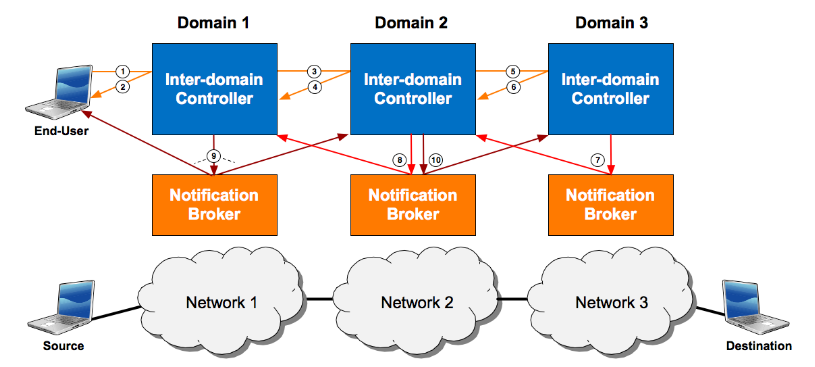
\includegraphics[width=0.6\textwidth]{figures/daisychain.png}
\caption{Daisy-chain model used by OSCARS for inter-domain circuit reservation, provisioning, and release}
\label{fig:daisychain}
\end{figure}

\paragraph{Path computation} In OSCARS v0.6, path computation
executed using ``atomic" Path Computation Engine (PCE) modules that can be
arbitrarily linked together. Each PCE module typically addresses a
specific constraint and prunes the graph accordingly. For example, a bandwidth PCE would discard all links that do not
have sufficient bandwidth, and a policy PCE would remove
all resources that the requester is not authorized to use.
While the PCE methods surveyed by Paolucci et al. \cite{6422287} are
for immediate-request paths, the OSCARS PCE supports
advance-reservation paths.


\subsection{Open Exchange Software Suite (OESS)}
\label{sec:OESS}

The Open Exchange Software Suite (OESS) is an OpenFlow
controller used to configure and control dynamic L2 paths
across a network of OpenFlow-enabled switches. OESS provides sub-second circuit provisioning, automatic circuit failover, per-interface permissions, and automatic per-VLAN
statistics.

\paragraph{OpenFlow path provisioning}
When a user wishes to provision an L2 path in OESS, the user must first select the endpoints (at least 2), rate, start time, duration, VLAN IDs, and optionally specify a path (with possibly a backup path) that connects all endpoints. In this context, endpoints are OpenFlow switch ports. For example, in Fig.~\ref{fig:oscarsoess}, consider the two numbered ports: port 19 of the DYNES switch in the University 1 network, and port 20 of the DYNES switch in the University 2 network. These two ports are the endpoints specified in a request for an end-to-end L2 path between the FDT hosts at University 1 and University 2.

Once the user has specified all the parameters in the request, the OESS UI sends the request to a Forwarding Controller. The Forwarding
Controller then calculates the \texttt{OFFlowMods}, which is a specification of the OpenFlow rules required to provision the path.
Each switch will receive at least 2 \texttt{OFFlowMods} (in cases of
multiPoint VLANs, there can be more than 2 \texttt{OFFlowMods}).
Each \texttt{OFFlowMod} is broken up into a \texttt{Match} and an \texttt{Action}.
The OpenFlow Match is applied to all packet headers, and
if a packet matches all of the fields in the OpenFlow \texttt{Match},
all of the OpenFlow \texttt{Actions} for the \texttt{OFFlowMod} are then
applied to the packet.

OESS has implemented a specific set
of OpenFlow \texttt{Matches} and \texttt{Actions}. All OESS \texttt{OFFlowMods}
for a VC consist of a \texttt{Match} that contains the input port
(\texttt{IN\_PORT}) and input VLAN ID (\texttt{DL\_VLAN}) fields. The
\texttt{Actions} consist of \texttt{SET\_VLAN\_ID} and OUTPUT (to a port)
actions. In some cases, the \texttt{STRIP\_VLAN} action is also used
(for untagged circuits). OESS uses NOX \cite{gude2008nox} to send \texttt{OFFlowMods} to the OpenFlow switches as shown in Fig.~\ref{fig:ControlPlane}.

In a network with QoS support, the controller would issue commands to configure filters, policing and scheduling in the OpenFlow switches so that flows do not violate the rates specified during path reservation. OpenFlow 1.3.0 supports QoS features, but the OESS implementation used in this study supported only OpenFlow 1.0 because Internet2 AL2S, for which OESS was initially designed, had only OpenFlow 1.0 switches when this study was carried out.

\paragraph{Topology discovery}
OESS learns the topology for its domain,
through a protocol similar to Link Layer Discovery Protocol (LLDP), called OpenFlow Discovery Protocol (OFDP) \cite{OFDP}.
OFDP functions by having the controller generate a packet
and send the packet out on every interface of an OpenFlow
switch using the \texttt{OFPacketOut} mechanism. The packet that
is sent out on each interface is tagged with the \texttt{DataPathID}
(a unique identifier for each OpenFlow Switch that is usually
based on a management MAC address) and number of the
interface on which the packet was sent. A rule is configured on
all switches to ``punt'' these topology-discovery packets to the
controller through an \texttt{OFPacketIn} event. The \texttt{OFPacketIn}
event sends the packet that arrived at the switch along with the
port and \texttt{DataPathID} of the switch that received the packet.
When this procedure occurs in both directions of an inter-switch link, an adjacency
is detected and OESS creates a link between the two devices on
the specified ports. OESS can also detects link failures and
node insertions, allowing for the OESS to automatically move
thousands of VLAN VCs with minimal human intervention.

% \paragraph{OESS software architecture}
% Fig.~\ref{fig:ControlPlane} shows the software architecture of OESS. OESS provisions an intra-domain circuit by using the NOX \cite{gude2008nox} API. NOX %is an OpenFlow controller that offers a programmatic interface to other controllers and applications. The module marked ``OSCARS''
% inside OESS is an interface to OSCARS. In addition to this interface, OESS has implemented
% a native module for NSI, the newer inter-domain control-plane protocol.

\begin{figure*}[htbp!]
\centering
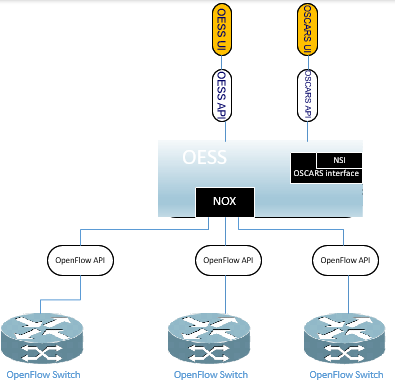
\includegraphics[width=0.6\textwidth]{figures/ControlPlane.PNG}
\caption{OESS software architecture}
\label{fig:ControlPlane}
\end{figure*}

\paragraph{OESS-OSCARS integration}
OESS includes an OSCARS interface module as shown in Fig.~\ref{fig:ControlPlane}. OESS automatically generates a
topology file for its domain and uploads it to the OSCARS
topology service as shown in Fig~\ref{fig:oscarsoess}. Only interfaces and VLAN IDs for which
users have granted OSCARS access appear in the OSCARS
topology file.

When a user requests an inter-domain circuit
via the OESS UI, the UI loads all topologies located in the
OSCARS topology service, and presents them to the user.
Once the endpoints have been selected and the user requests
that a VC be provisioned, the OESS UI submits a request to
OSCARS via the OSCARS SOAP API on behalf of the user.
At this point, the request has been turned over to OSCARS to
complete its path computation, and inform the other domains
of the request. When it is time for OSCARS to provision the
circuit in the local domain, it contacts the Path Setup Service
(PSS). When OESS is deployed in a domain, the OSCARS
PSS is replaced with the OESS PSS. The OESS PSS takes
the provisioning request from OSCARS, as shown in Fig~\ref{fig:oscarsoess}, and provisions an
OpenFlow path as described earlier. The OESS then reports the
success or failure of the provisioning procedure to OSCARS.
In cases where a user request for an inter-domain VC is sent
directly to OSCARS, the OESS PSS is nevertheless involved
to check the validity of the VC request and to carry out the
OpenFlow path provisioning.

\begin{figure}
\centering
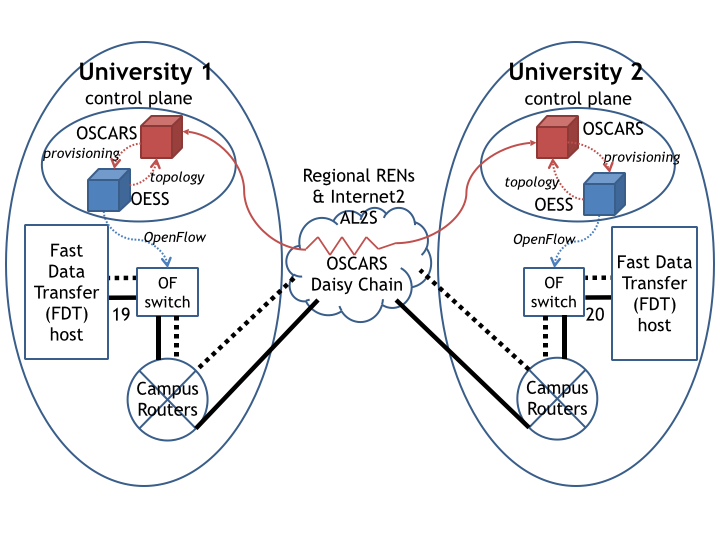
\includegraphics[width=0.6\textwidth]{figures/oscarsoess.png}
\caption{OSCARS and OESS integration}
\label{fig:oscarsoess}
\end{figure}
